\chapter{Esercizio 1}

\section{Multiplexer 16:1}
Un multiplexer è una \textbf{macchina combinatoria}, ovvero una macchina la cui uscita in un determinato istante di tempo dipende solo dall'ingresso nel medesimo istante, e quindi realizza una funzione del tipo:
\begin{equation*}
    U = f(I)
\end{equation*}
dove $I$ e $U$ rappresentano rispettivamente gli insiemi limitati dei valori di ingresso e di uscita.\\
Il Multiplexer realizza una connessione \textit{n:1}, ovvero connette $n$ sorgenti a un'unica destinazione sulla base di segnali di selezione.\\
Un \textbf{Multiplexer lineare} è composto da $n$ segnali in ingresso e $n$ segnali di selezione. Tale dispositivo convoglia uno specifico segnale in ingresso verso l'uscita solo se il corrispondente segnale di selezione è alto. Uno svantaggio di un dispositivo di questo tipo è il numero eccessivo di fili per i segnali di selezione. Per risolvere ciò si può aggiungere un \textbf{Decoder}, un altro dispositivo notevole, che riceve in ingresso una parola codice di $n$ bit e presenta in uscita la sua rappresentazione decodificata di \(2^n\) bit.\\
Unendo un Multiplexer lineare a un Decoder, l'architettura diventa quella in figura, e si ottiene un componente definito \textbf{Multiplexer indirizzabile}, che diversamente da quello lineare, prende solo 2 segnali di selezione in ingresso. Un MUX indirizzabile è a sua volta una macchina notevole, caratterizzata da \(2^n\) ingressi, $n$ ingressi di selezione e un'unica uscita.
\begin{figure}[H]
	\centering
	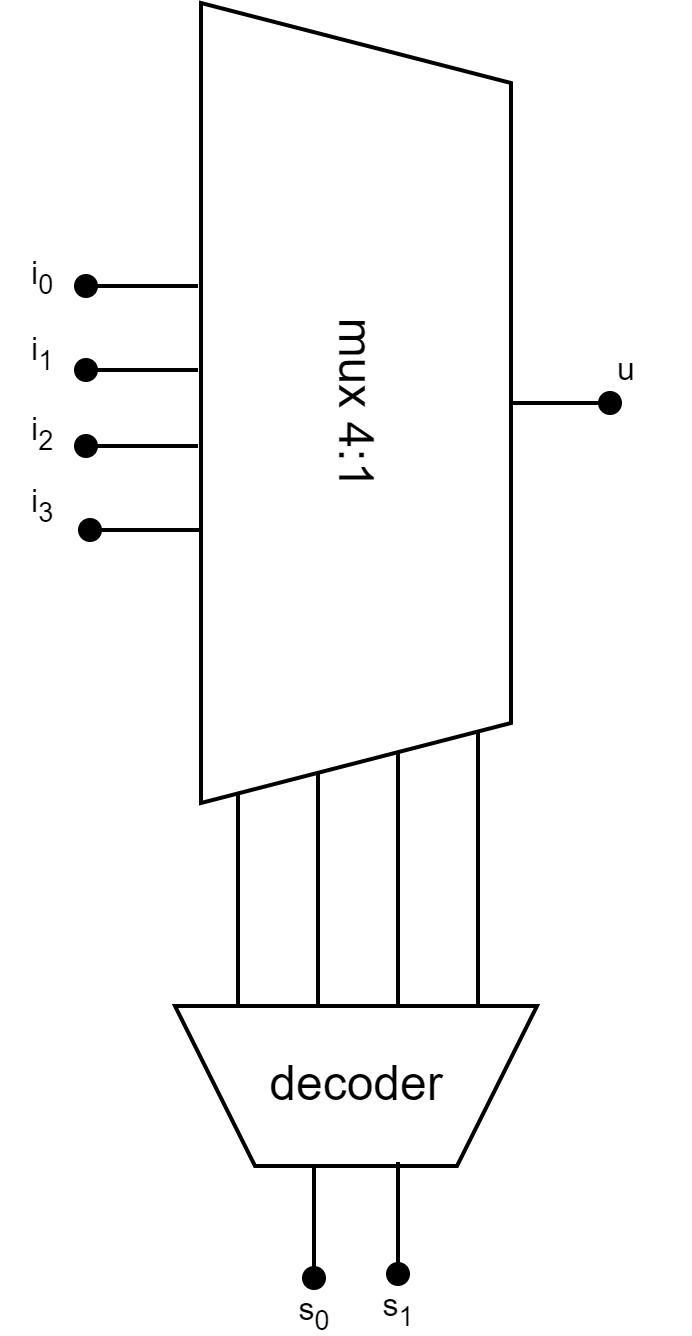
\includegraphics[width=0.4\textwidth]{img/mux_indirizz}
	\caption{multiplexer indirizzabile}
	\label{mux_16:1} 
\end{figure}
Si vuole ora progettare un multiplexer indirizzabile 16:1, utilizzando un approccio per composizione, a partire da multiplexer 4:1.\\
Tale multiplexer è rappresentato di seguito.
\begin{figure}[H]
	\centering
	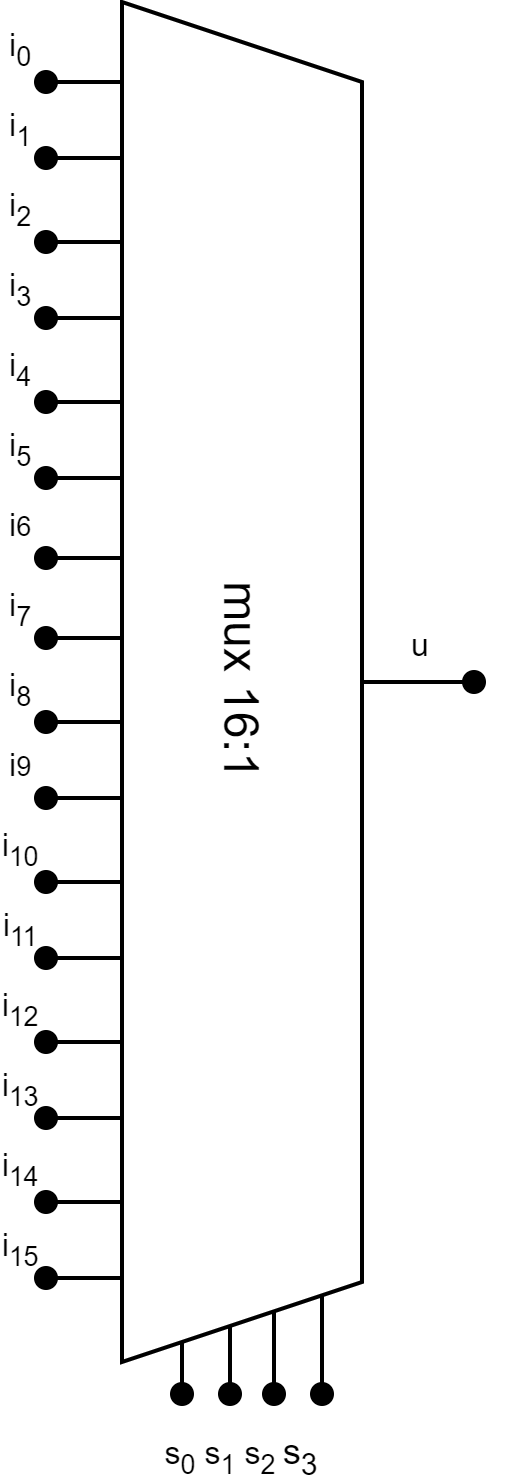
\includegraphics[width=0.3\textwidth]{img/mux_16-1}
	\caption{multiplexer 16:1}
	\label{mux_16:1} 
\end{figure}

\subsection{Progetto e architettura}
Dapprima si utilizza un approccio per composizione per realizzare un multiplexer 4:1 con multiplexer 2:1.\\
\begin{figure}[H]
	\centering
	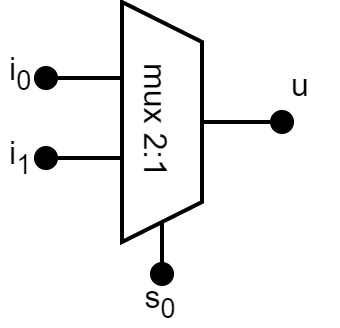
\includegraphics[width=0.3\textwidth]{img/mux_2-1}
	\caption{multiplexer 2:1}
	\label{mux_2:1} 
\end{figure}
Il primo componente che si realizza è un multiplexer 2:1, caratterizzato dalla seguente tabella di verità:
\begin{table}[h!]
    \centering
    \begin{tabular}{||c|c|c||c||}
        \hline
        \hline
         $\mathbf{s_0}$ & $\mathbf{i_1}$ & $\mathbf{i_0}$ & $\mathbf{u}$\\
         \hline
         0 & 0 & 0 & 1 \\
         \hline
         0 & 0 & 1 & 1 \\
         \hline
         0 & 1 & 0 & 0 \\
         \hline
         0 & 1 & 1 & 1 \\
         \hline
         1 & 0 & 0 & 0 \\
         \hline
         1 & 0 & 1 & 0 \\
         \hline
         1 & 1 & 0 & 1 \\
         \hline
         1 & 1 & 1 & 1 \\
         \hline
         \hline 
    \end{tabular}
    \caption{Tabella di verità di un Mux 2:1}
    \label{tab:mux_2:1}
\end{table}
    
%\begin{figure}[H]
%	\centering
%	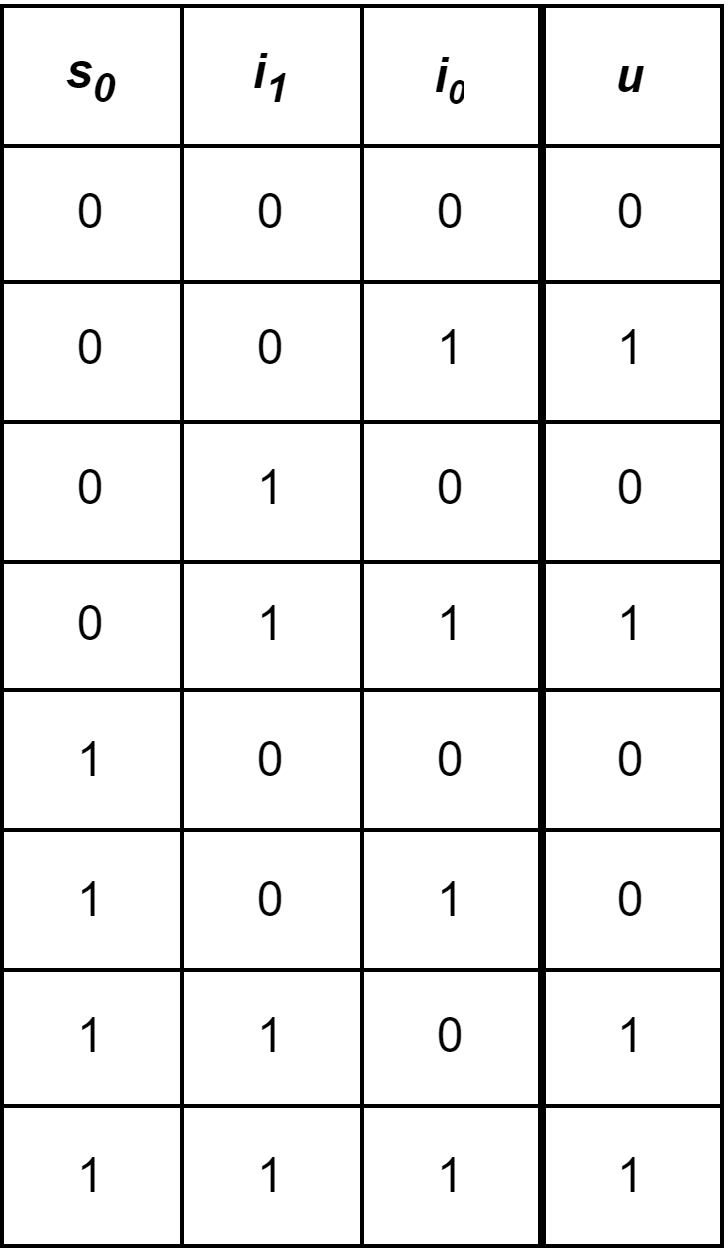
\includegraphics[width=0.3\textwidth]{img/tabVeritaMux_2_1}
%	\caption{Tabella di verità di un Mux 2:1}
%	\label{tab_mux_2:1} 
%\end{figure}
da cui si ottiene l'equazione:
\begin{center}
    \begin{equation*}
          u = (i_0 \text{ AND } \bar{s_0}) \text{ OR } (i_1 \text{ AND } s_0)
    \end{equation*}
\end{center}
Il successivo componente da costruire è un multiplexer 4:1.
\begin{figure}[H]
	\centering
	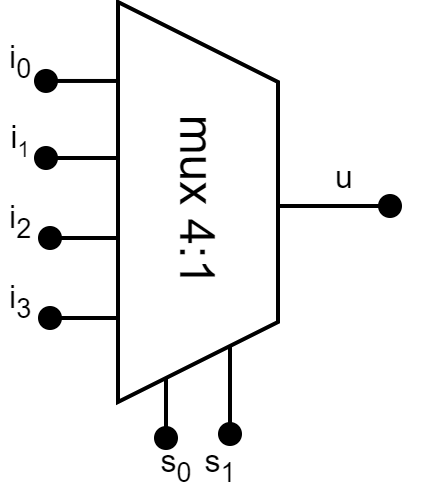
\includegraphics[width=0.3\textwidth]{img/mux_4-1}
	\caption{multiplexer 4:1}
	\label{mux_4:1} 
\end{figure}
Per composizione, a partire da 3 multiplexer 2:1, si può ottenere un multiplexer 4:1
\begin{figure}[H]
	\centering
	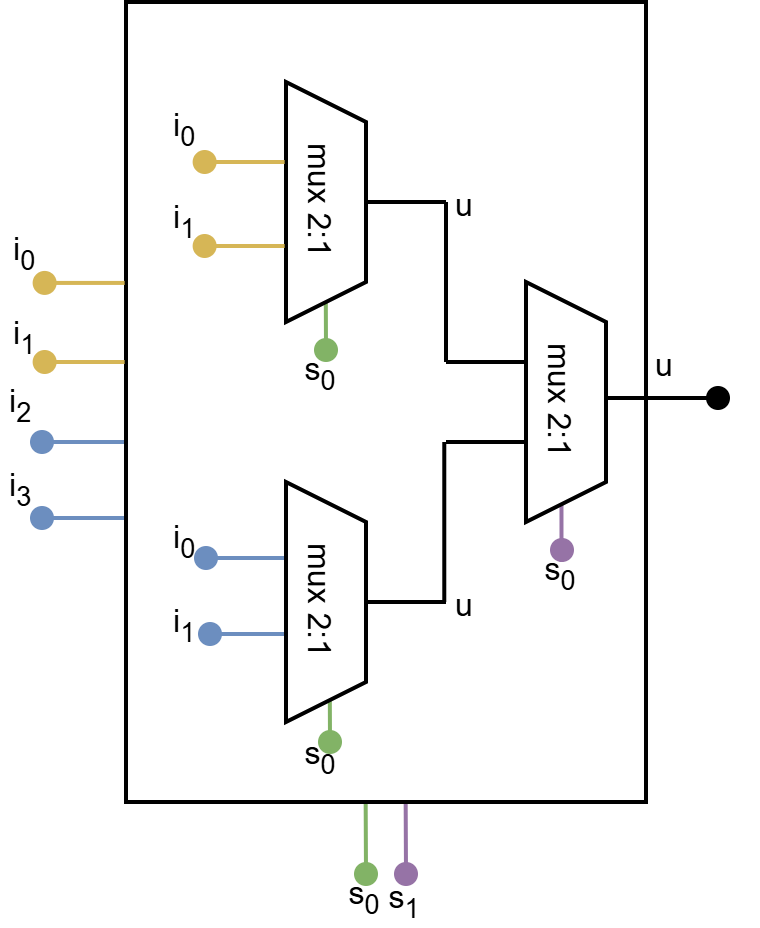
\includegraphics[width=0.7\textwidth]{img/mux_4-1_comp}
	\caption{multiplexer 4:1 per composizione di multiplexer 2:1}
	\label{mux_4:1_comp} 
\end{figure}
I 4 ingressi entrano in due multiplexer 2:1, che prendono due ingressi e producono un'uscita ciascuno; tali uscite vengono immesse nel terzo multiplexer, che produrrà l'unico output finale. Concettualmente, si divide la selezione in ingresso al multiplexer esterno in due parti:
\begin{itemize}
    \item la parte meno significativa (indicata dal colore verde) \(s_0\), viene posta in ingresso ai multiplexer del primo stadio e seleziona per ciascuno un filo in uscita;
    \item la parte più significativa (indicata dal colore viola) \(s_1\) entra nel multiplexer del secondo stadio e decide quale dei due fili, provenienti dai due blocchi precedenti, sarà immessa in uscita.
\end{itemize}
In maniera analoga si procede con la progettazione del multiplexer 16:1.\\
Anche in questo caso, sono stati usati dei colori per identificare i collegamenti tra le componenti.
\begin{figure}[H]
	\centering
	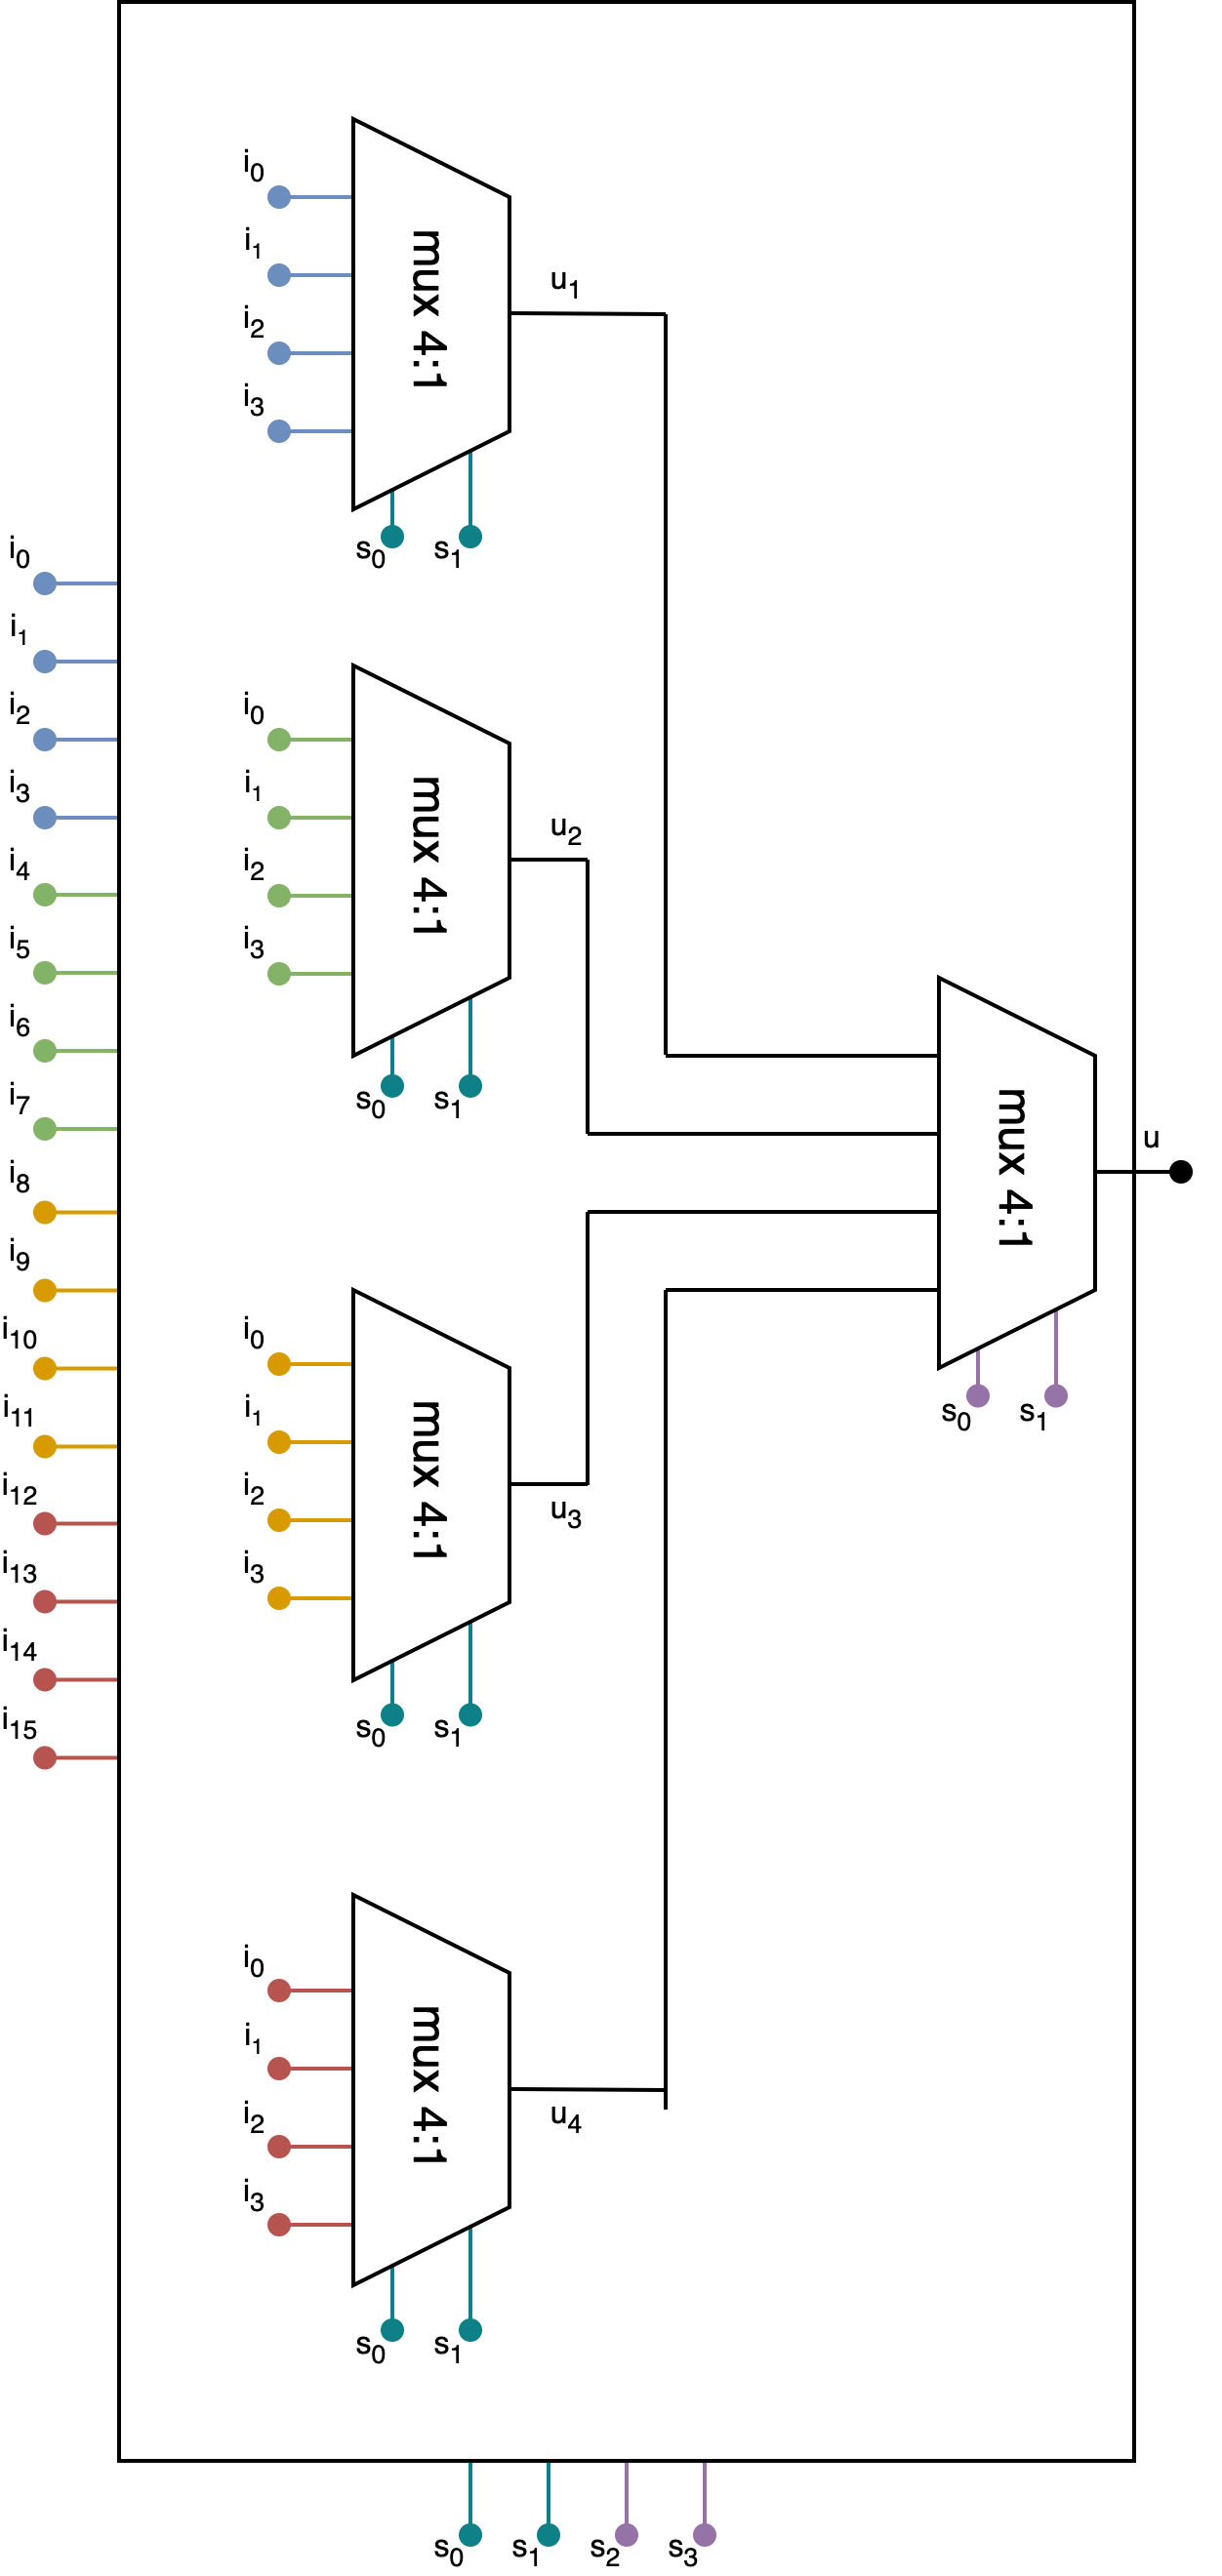
\includegraphics[width=0.7\textwidth]{img/mux_16-1_composizione}
	\caption{multiplexer 16:1 per composizione di multiplexer 4:1}
	\label{mux_16:1_comp} 
\end{figure}


\subsection{Implementazione}
Per l'implementazione si procede con un approccio di tipo strutturale, iniziando quindi dalla codifica del multiplexer 2:1, e, a partire da questo si compongnono dispositivi sempre più complessi fino ad arrivare all'obiettivo del multiplexer 16:1.
\paragraph{Mux 2:1} Di seguito il codice riguardante il Mux 2:1.
\begin{code}
    \inputminted[frame=lines, framesep=2mm, baselinestretch=1.2, bgcolor=LightGray, fontsize=\footnotesize, linenos]{vhdl}{vhdl_files/mux_2_1.vhdl}
    \caption{Multiplexer 2:1 in VHDL}
    \label{lst:mux_2_1}
\end{code}
L'interfaccia del componente ha come ingressi \texttt{i0} ed \texttt{i1}, come selezione \texttt{s0} e come uscita \texttt{u}.\\
Al seguito della definizione dell'interfaccia, si definisce il comportamento dell'entità, che risponde alla tabella della verità \ref{tab:mux_2:1}.\\
\paragraph{Mux 4:1} Si prosegue con il Mux 4:1. \\
Come anticipato, viene costruito a partire da tre mux 2:1.
\begin{code}
    \inputminted[frame=lines, framesep=2mm, baselinestretch=1.2, bgcolor=LightGray, fontsize=\footnotesize, linenos]{vhdl}{vhdl_files/mux_4_1.vhdl}
    \caption{Multiplexer 4:1 in VHDL}
    \label{lst:mux_4_1}
\end{code}
%spiegazione codice 4:1
In quest'entità, l'interfaccia è dichiarata come segue:
\begin{itemize}
    \item Il parametro \texttt{i} vettore di 4 elementi, ognuno corrispondente ad un ingresso del mux 4:1.
    \item Il parametro \texttt{s} vettore di 2 elementi, ognuno corrispondente ad un ingresso di selezione.
    \item Il parametro \texttt{u} corrispondente all'uscita del multiplexer.
\end{itemize}
A seguire si definisce la struttura del mux 4:1, utilizzando mux 2:1 come componenti. \\
Con il ciclo \texttt{for}, vengono stanziati i primi due mux 2:1, i quali riceveranno in ingresso rispettivamente, gli ingressi del mux 4:1 e la loro uscita è il vettore d'appoggio \texttt{u\_mid}, il quale è talvolta l'ingresso del terzo mux 2:1.
\paragraph{Mux 16:1} In maniera analoga si procede con la costruzione del mux 16:1.
Il codice è il seguente:
\begin{code}
    \inputminted[frame=lines, framesep=2mm, baselinestretch=1.2, bgcolor=LightGray, fontsize=\footnotesize, linenos]{vhdl}{vhdl_files/mux_16_1.vhdl}
    \caption{Multiplexer 16:1 in VHDL}
    \label{lst:mux_16_1}
\end{code}

\subsection{Simulazione}
Per la simulazione, vi è la necessità di un testbench, il quale generiamo in maniera automatica tramite software appositi.\\
In tale progetto la generazione viene effettuata tramite ChatGPT ed il codice è il seguente:
\begin{code}
    \inputminted[frame=lines, framesep=2mm, baselinestretch=1.2, bgcolor=LightGray, fontsize=\footnotesize, linenos]{vhdl}{vhdl_files/tb_mux_16_1.vhdl}
    \caption{Testbench multiplexer 16:1 in VHDL}
    \label{lst:tb_mux_16_1}
\end{code}
 Una volta generato ciò, utilizzando i software GHDL e GTKWAVE, vengono eseguiti i seguenti comandi:
 \begin{figure}[H]
	\centering
	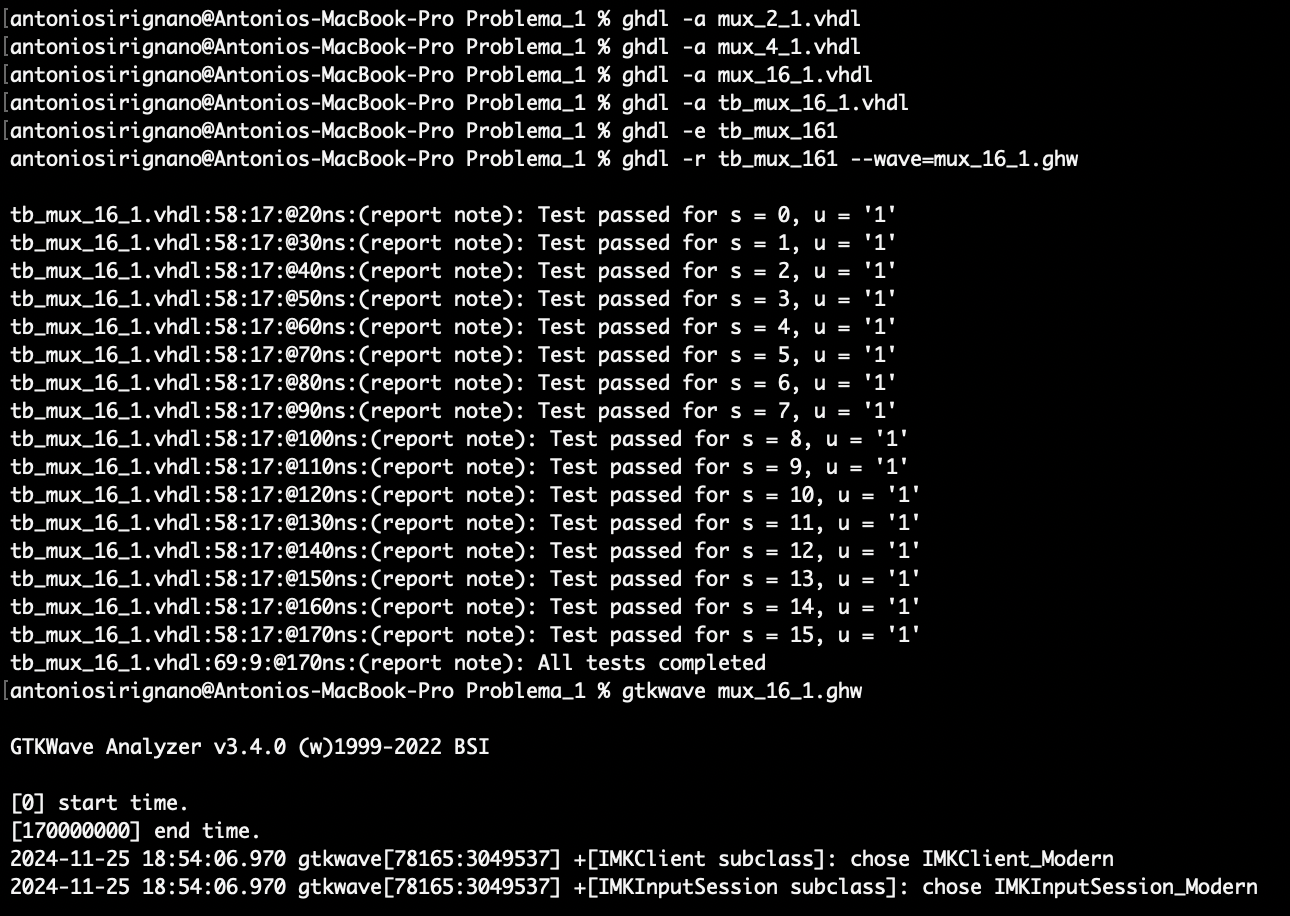
\includegraphics[width=1\textwidth]{img/commands_sim_16_1}
	\caption{Comandi per la simulazione}
	\label{comandi_sim_mux_16:1} 
\end{figure}
Con l'esecuzione dell'ultimo comando, vi si apre una nuova finestra che permette la visualizzazione delle onde:
 \begin{figure}[H]
	\centering
	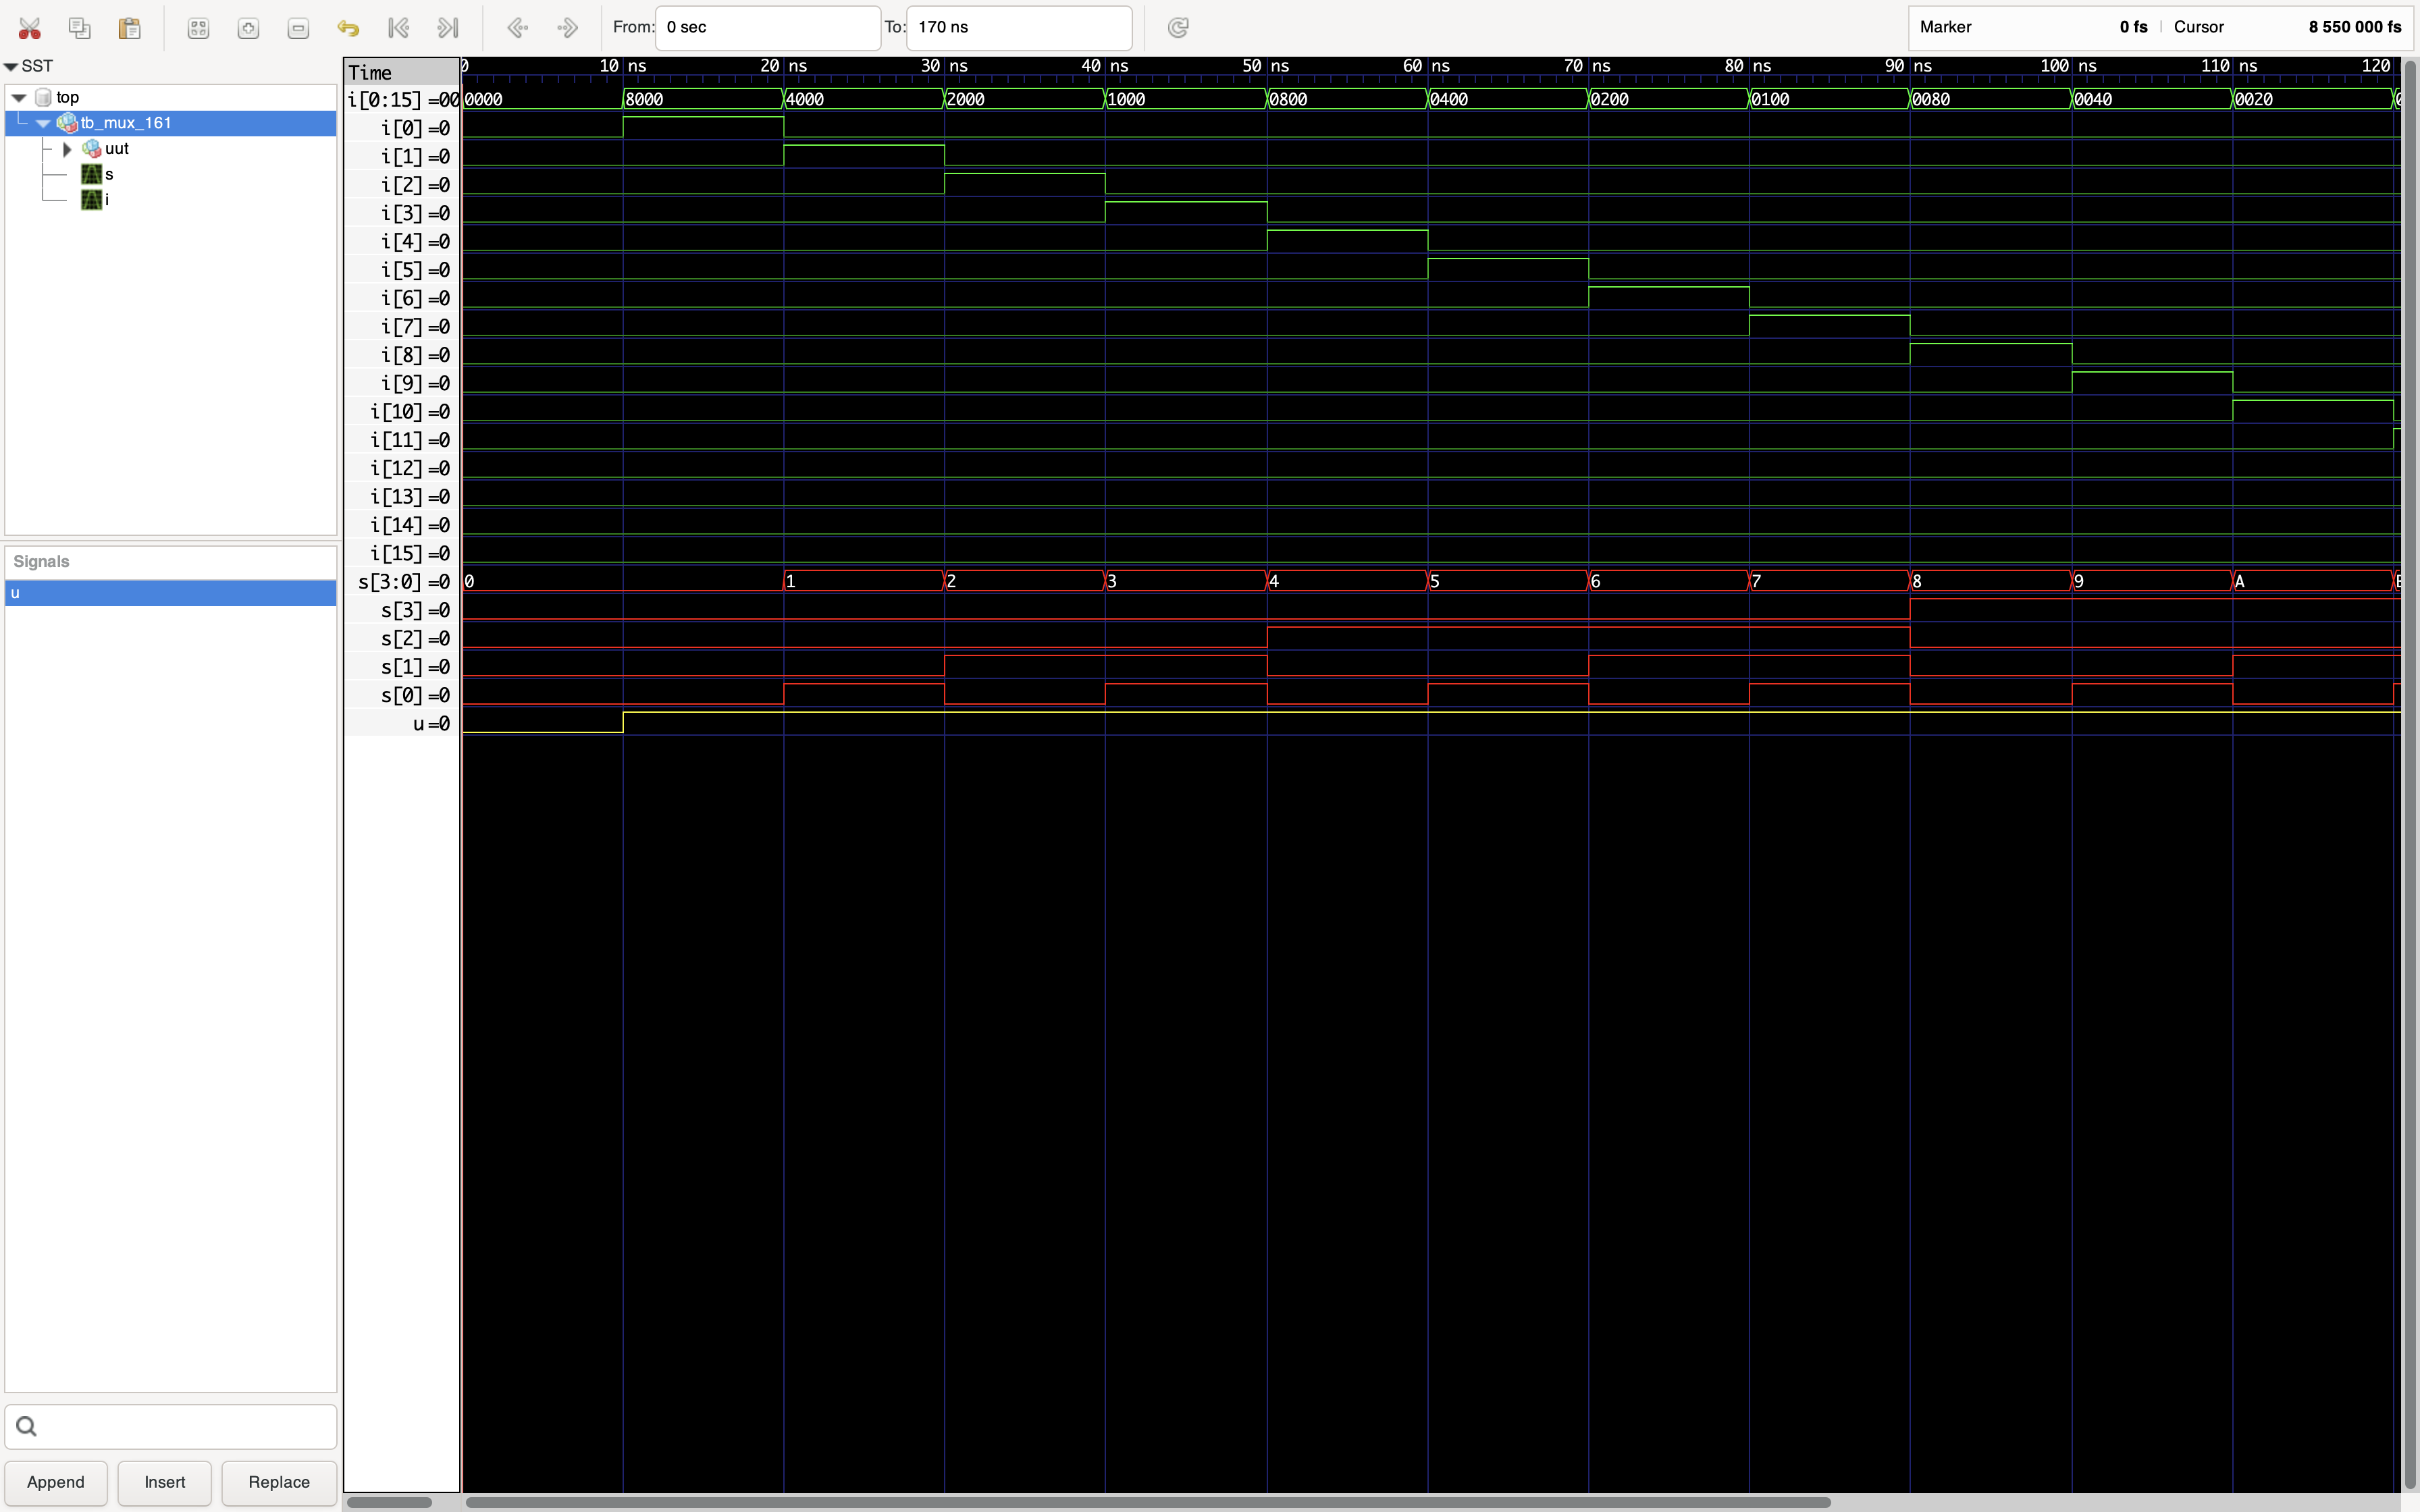
\includegraphics[width=1\textwidth]{img/waves_sim_16_1}
	\caption{Risultati della simulazione: waveform}
	\label{comandi_sim_mux_16:1} 
\end{figure}

\section{Rete di interconnessione a 16 ingressi e 4 uscite}
Una rete di interconnessione è è un tipo di rete di commutazione che permette di instradare i segnali da un insieme di ingressi a un insieme più ridotto di uscite. Tale rete può essere progettata attraverso un adeguato utilizzo di Multiplexer e Demultiplexer. \\
Nel caso in esame, si vuole progettare una rete che prenda 16 ingressi e restituisca 4 uscite. Si utilizza anche in questo caso un approccio per composizione, a partire dal Multiplexer 16:1 implementato nell'esercizio precedente, la cui uscita sarà posta in ingresso a un Demultiplexer 1:4.\\
La rete complessiva sarà fatta in questo modo:
 \begin{figure}[H]
	\centering
	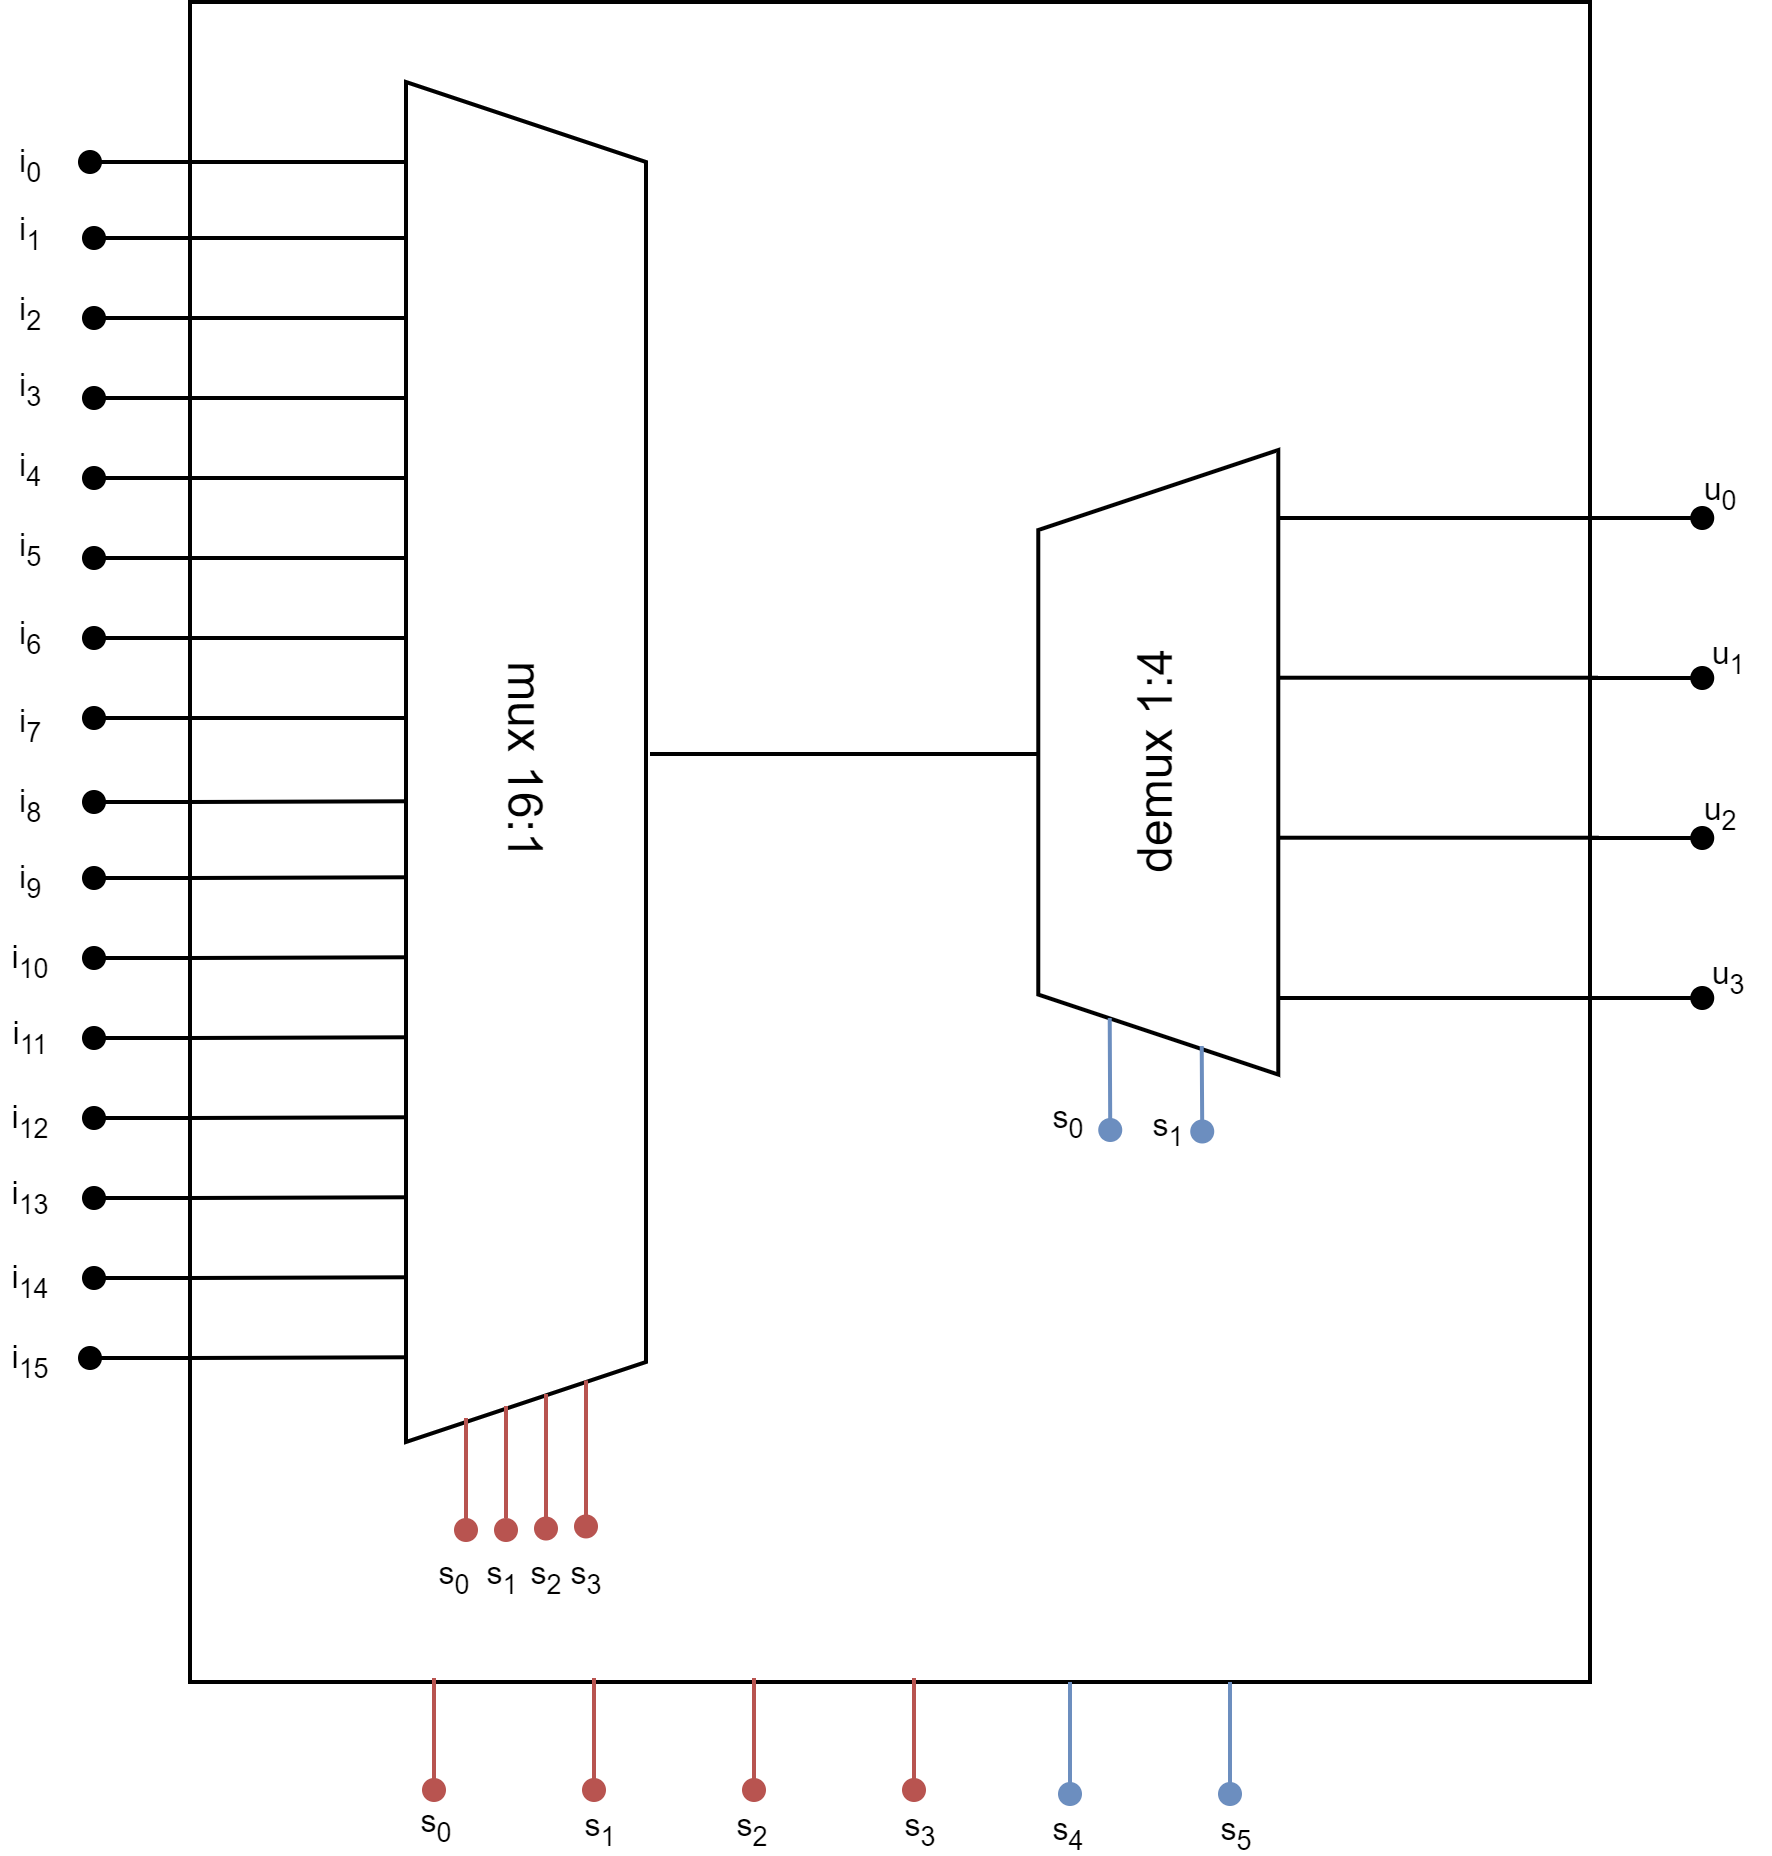
\includegraphics[width=1\textwidth]{img/Rete_interconn}
	\caption{Rete di interconnesione}
	\label{Demux 1:2} 
\end{figure}


\subsection{Progettazione}
 Anche in questo caso, prima di procedere all'implementazione della rete nel complesso, si costruisce il Demultiplexer 4:1 a partire da Demultiplexer 2:1.\\
Un Demultiplexer $1:u$ è un dispositivo che prende un solo segnale di ingresso, due segnali di selezione e a partire da essi restituisce $u$ uscite. \\
Un Demultiplexer 2:1 è un dispositivo fatto in questo modo:
 \begin{figure}[H]
	\centering
	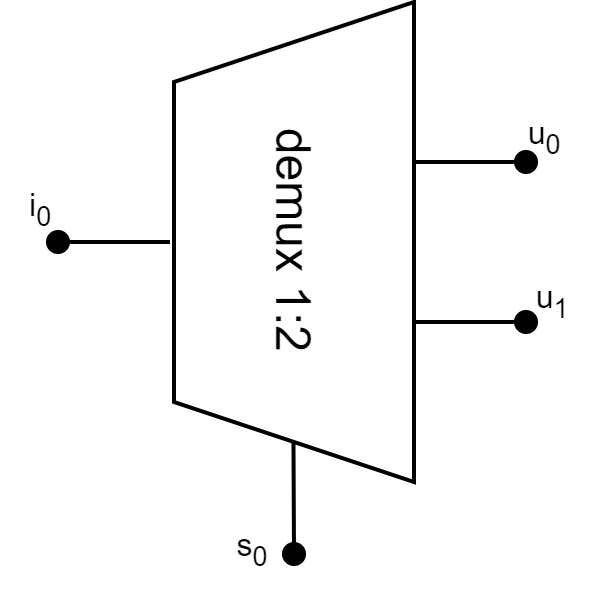
\includegraphics[width=0.5\textwidth]{img/demux_1_2}
	\caption{Demux 1:2}
	\label{Demux 1:2} 
\end{figure}
Tale componente è caratterizzato dalla seguente tabella di verità:
\begin{table}[H]
    \centering
    \begin{tabular}{||c|c|c||c||}
        \hline
        \hline
         $\mathbf{s_0}$ & $\mathbf{i_0}$ & $\mathbf{u_0}$ & $\mathbf{u_1}$\\
         \hline
         0 & 0 & 0 & 0 \\
         \hline
         0 & 1 & 1 & 0 \\
         \hline
         1 & 0 & 0 & 0 \\
         \hline
         1 & 1 & 0 & 1 \\
         \hline
         \hline 
    \end{tabular}
    \caption{Tabella di verità di un Demux 2:1}
    \label{tab:demux_2:1}
\end{table}
Da cui si ricavano le seguenti equazioni relative alle uscite:
\begin{equation*}
    \begin{aligned}
          u_0 = (i_0 \text{ AND } \bar{s_0})\\
          u_1 = (i_0 \text{ AND } {s_0})
    \end{aligned}
    \end{equation*}
A partire dalla composizione di dispositivi di questo tipo, si può realizzare un Demultiplexer 1:4, come rappresentato in figura.
\begin{figure}[H]
	\centering
	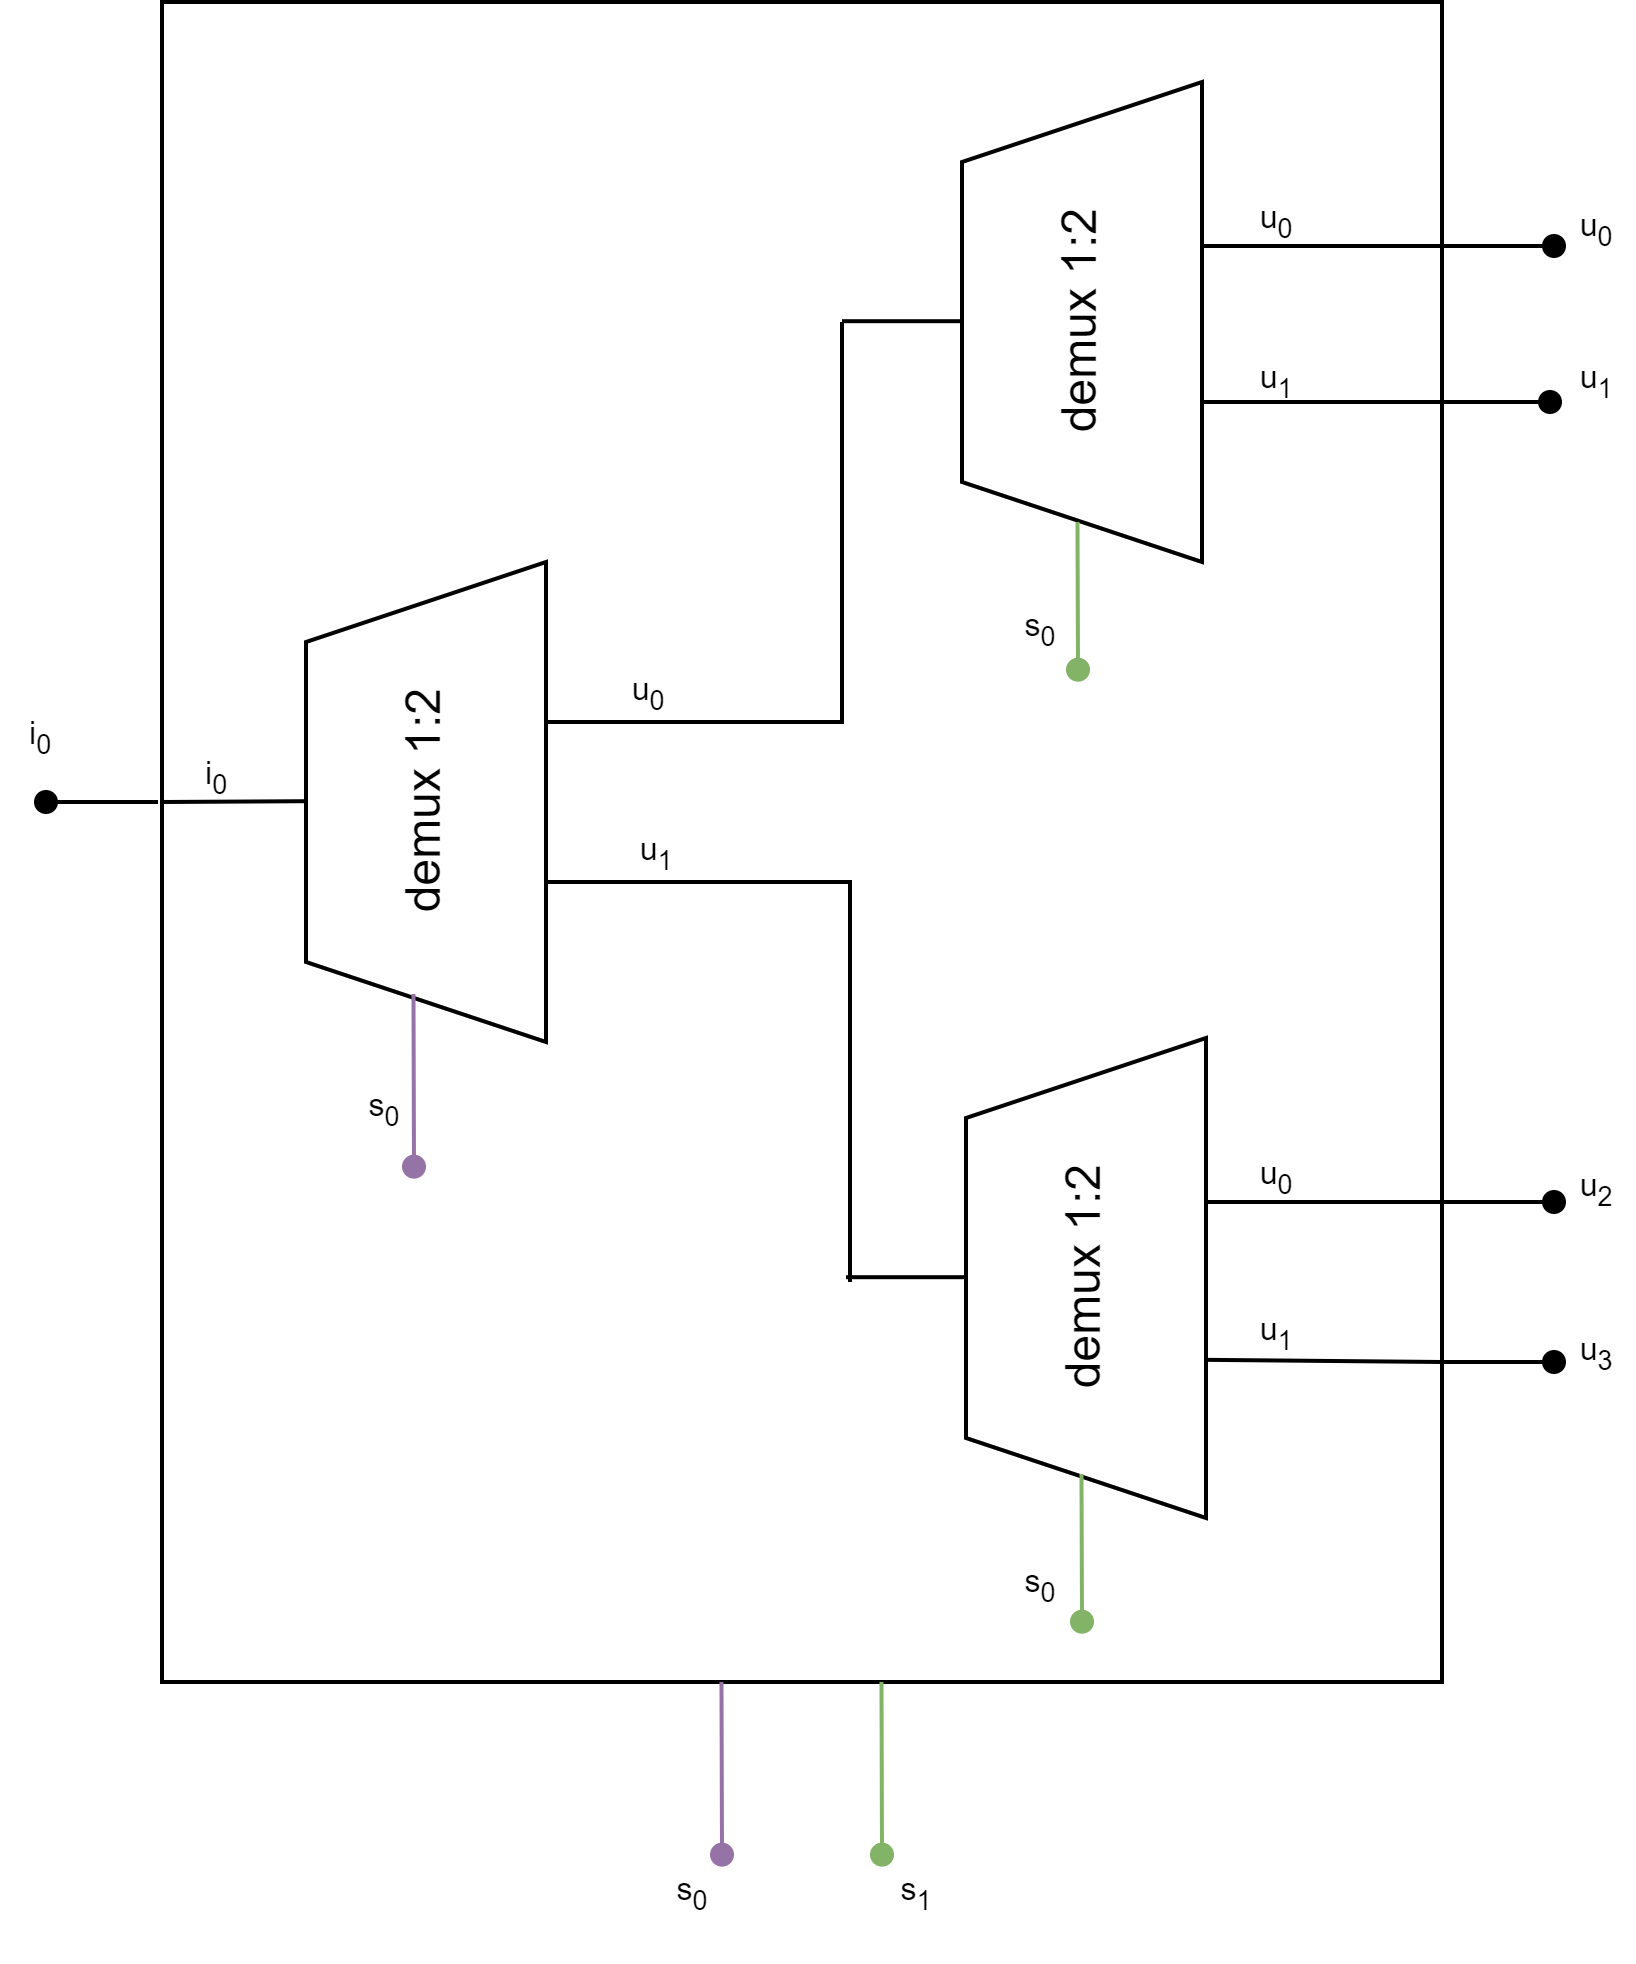
\includegraphics[width=0.8\textwidth]{img/demux_1_4}
	\caption{Demux 1:4 composto a partire da Demux 1:2}
	\label{Demux 1:2} 
\end{figure}
Utilizzando il Demultiplexer appena progettato, al cui ingresso si fa corrispondere l'uscita del Multiplexer 16:1, progettato nell'esercizio precedente, si ottiene la rete di interconnessione, così formata:
\begin{figure}[H]
	\centering
	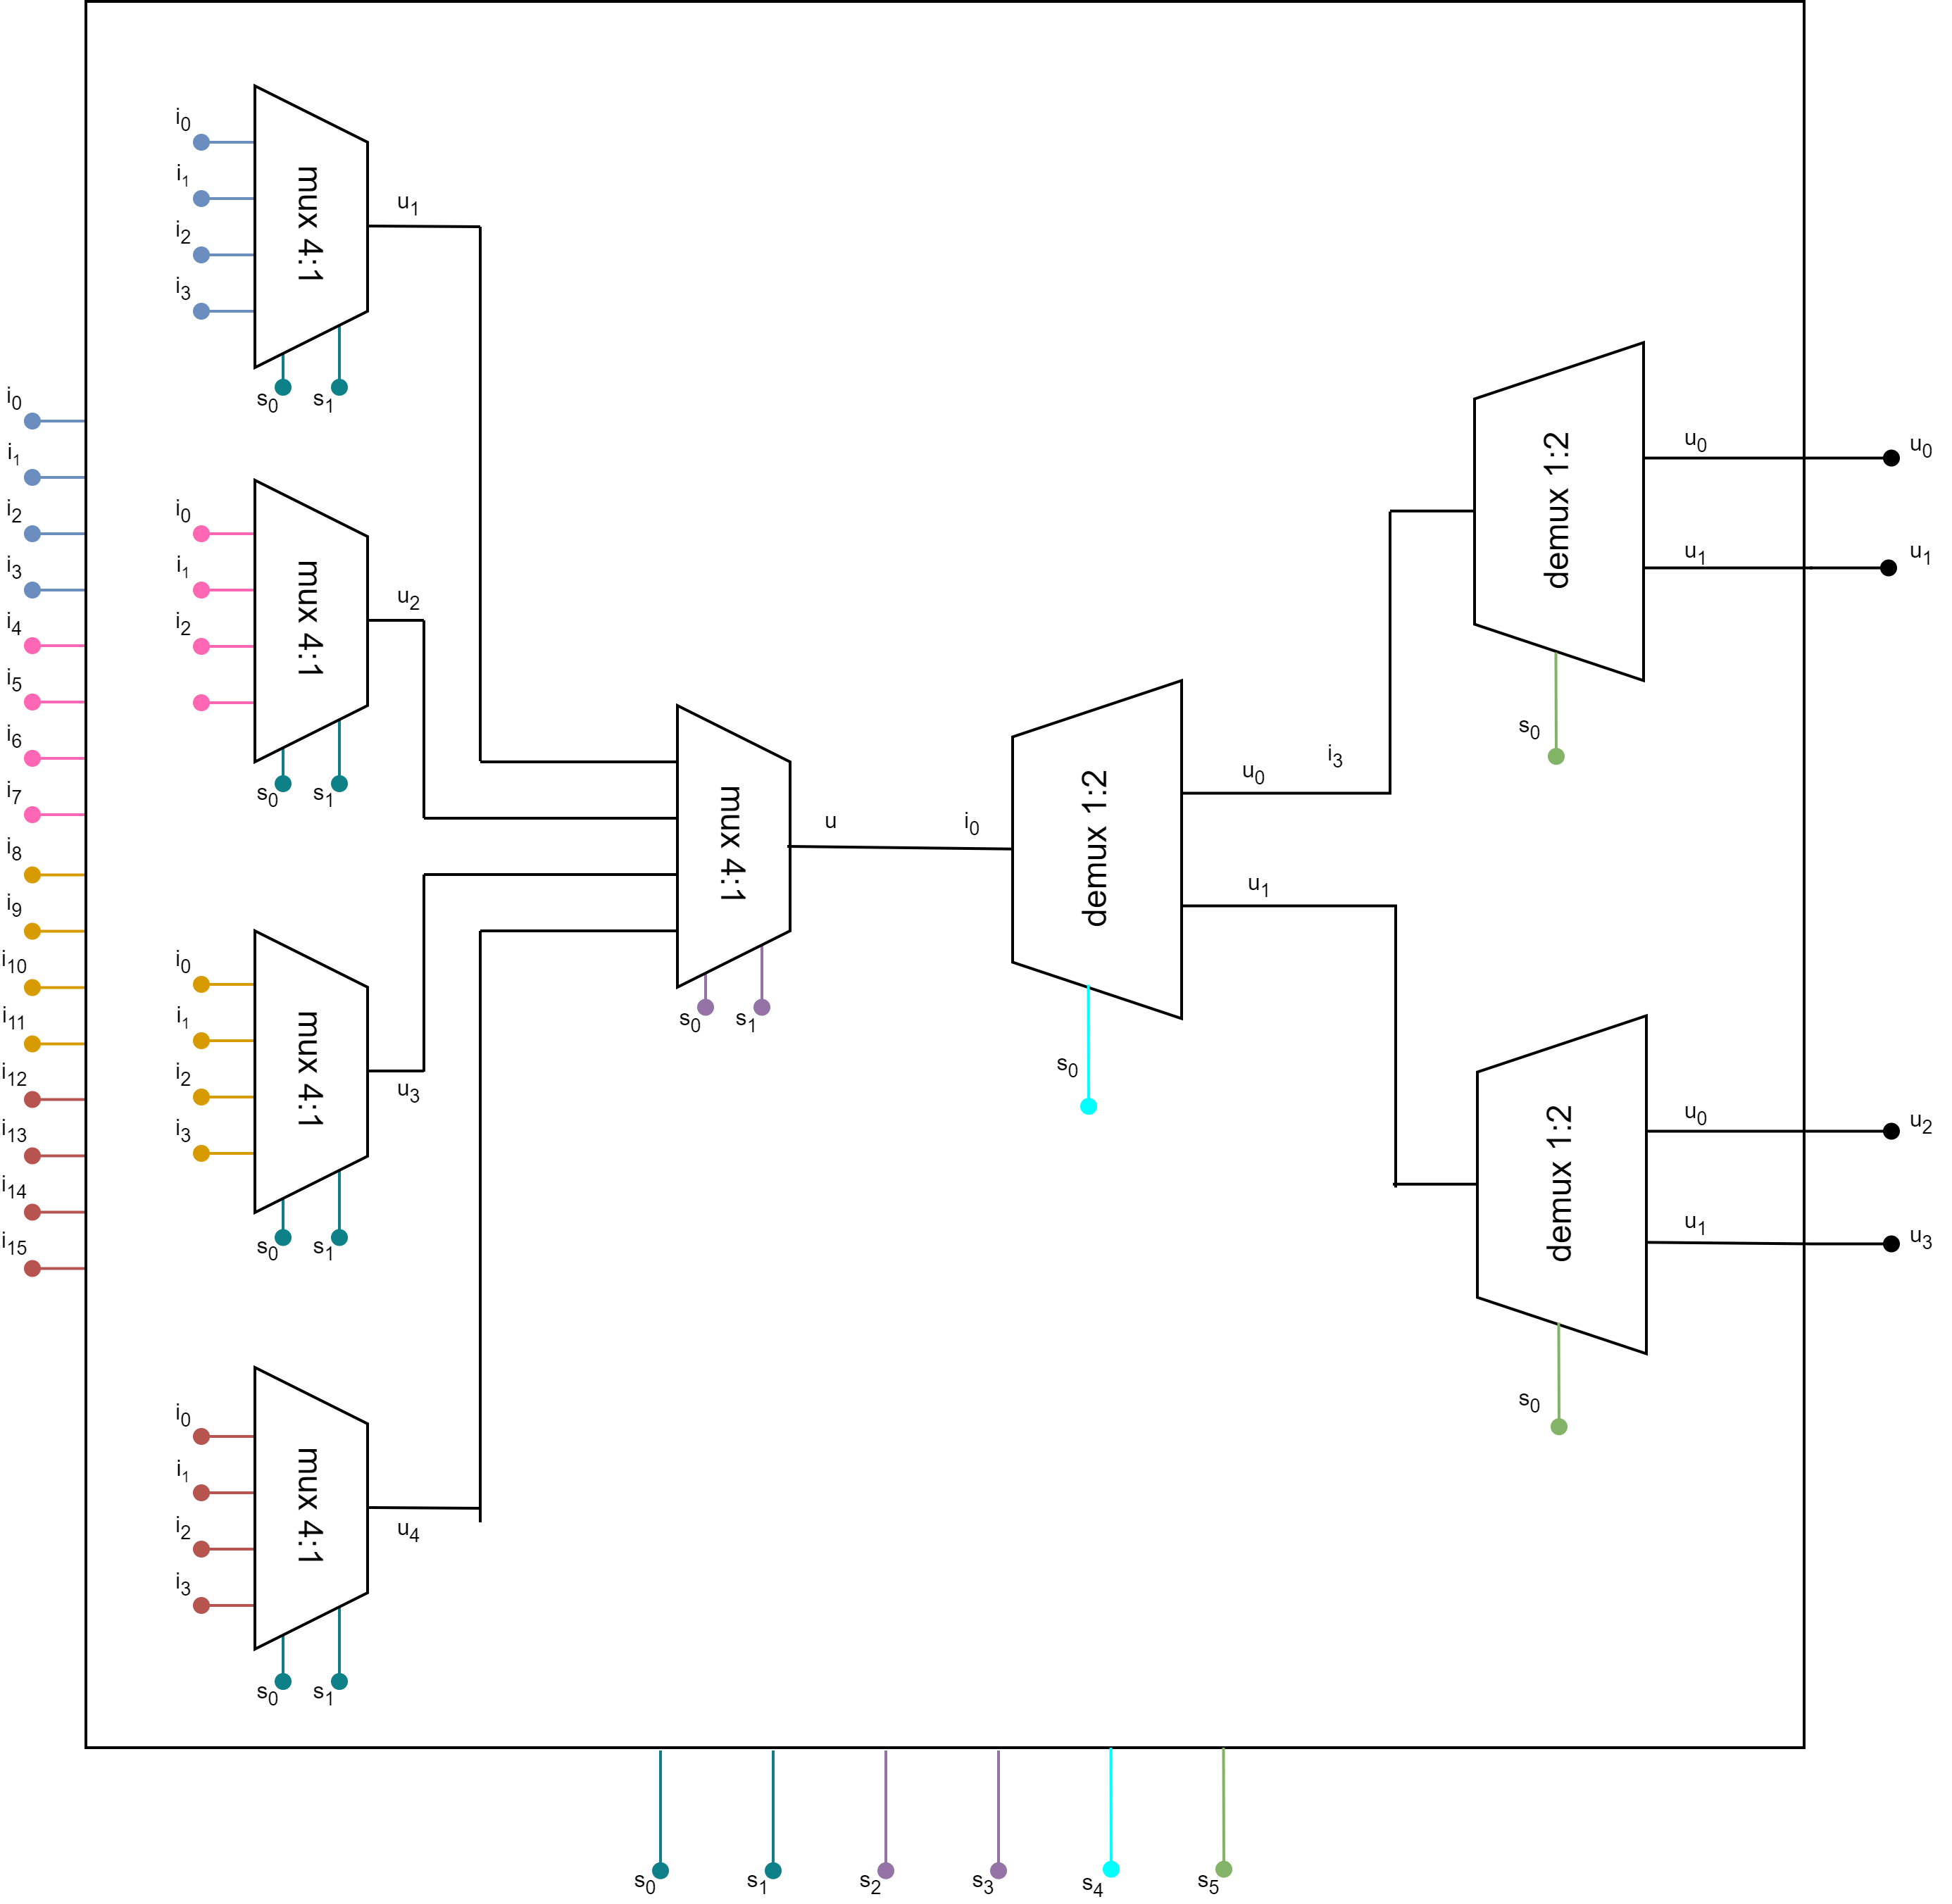
\includegraphics[width=1\textwidth]{img/ReteInterconn_composta}
	\caption{Rete di interconnessione: funzionamento interno}
	\label{Demux 1:2} 
\end{figure}
Nell'immagine, i colori sono stati usati per rendere più chiari i collegamenti tra segnali.

\subsection{Implementazione}
%da fare
\subsection{Simulazione}
%da fare
\section{Implementazione su board del punto precedente}
%da fare appena si ha la board

\chapter{Esercizio 2 - Sistema ROM+M}
Il sistema che si vuole costruire consiste in due elementi principali: una ROM (Read-Only-Memory) puramente combinatoria e una macchina combinatoria M, che esegue una trasformazione sui dati letti da M e li pone in uscita. La ROM si compone di 16 locazioni di memoria, ciascuna contenente una stringa di 8 bit. Il sistema prende in ingresso un indirizzo di 4 bit, che permetterà di accedere a una delle locazioni della ROM; il dato in tale locazione viene posto in uscita alla ROM, e quindi in ingresso alla macchina M. La macchina M deve effettuare una trasformazione sulla stringa di 8 bit, in modo da restituire in uscita una stringa di 4 bit. La trasformazione scelta consiste nel sommare i 4 bit più significativi della stringa con i 4 bit meno significativi, la stringa di 4 bit risultante sarà restituita come uscita all'intero sistema.
\begin{figure}[H]
	\centering
	\includegraphics[width=0.8\textwidth]{img/rom_M_black_box}
	\caption{ROM + M}
	\label{Rom_M} 
\end{figure}
\section{Progettazione}
La progettazione consiste nella realizzazione dei due componenti fondamentali del sistema: ROM e M. 
\section{Implementazione}
Dapprima si implementa la ROM, in cui sono memorizzati 16 elementi, ciascuno da 8 bit. Il codice sottostante crea l'entità ROM, al cui ingresso è presente un vettore da 4 bit di $std\_logic$ che rappresenta l'indirizzo, e in uscita restituisce un vettore di 8 bit. Vengono poi definite le stringhe di bit contenute nella ROM. Nel processo main, si pone in uscita l'elemento corrispondente alla locazione address.\\
%\paragraph{Mux 2:1} Di seguito il codice riguardante il Mux 2:1.
\begin{code}
    \inputminted[frame=lines, framesep=2mm, baselinestretch=1.2, bgcolor=LightGray, fontsize=\footnotesize, linenos]{vhdl}{vhdl_files/ROM.vhd}
    \caption{Implementazione ROM in VHDL}
    \label{lst:ROM}
\end{code}
Si procede poi con l'implementazione del componente M, che effettua la trasformazione.
\begin{code}
    \inputminted[frame=lines, framesep=2mm, baselinestretch=1.2, bgcolor=LightGray, fontsize=\footnotesize, linenos]{vhdl}{vhdl_files/M.vhd}
    \caption{Macchina M}
    \label{lst:M}
\end{code}
Nel processo si pone come uscita della macchina la somma tra i bit più significativi dell'ingresso (dal bit 7 al 4) e dei bit meno significativi (dal bit 3 allo 0).\\
Le due componenti sono parte del sistema S che è così implementato:
\begin{code}
    \inputminted[frame=lines, framesep=2mm, baselinestretch=1.2, bgcolor=LightGray, fontsize=\footnotesize, linenos]{vhdl}{vhdl_files/ROMplusM.vhd}
    \caption{Sistema S}
    \label{lst:S}
\end{code}
Tale sistema è stato costruito come structural: sono stati dichiarati i componenti, e ne sono state definite le istanze. Si è utilizzato un segnale di supporto $u0$, che funge da segnale intermedio tra l'uscita della ROM e l'ingresso della macchina. \\
Si osserva lo schematic fornito dall'ambiente di sviluppo Vivado:
\begin{figure}[H]
	\centering
	\includegraphics[width=1\textwidth]{img/ROM_plus_M}
	\caption{Schematic di S}
	\label{SchemS} 
\end{figure}

\section{Simulazione}
Per procedere alla simulazione si realizza un testbench, con diversi casi di test, che permettano di osservare il comportamento del sistema.
\begin{code}
    \inputminted[frame=lines, framesep=2mm, baselinestretch=1.2, bgcolor=LightGray, fontsize=\footnotesize, linenos]{vhdl}{vhdl_files/ROMplusM_tb.vhd}
    \caption{Testbench}
    \label{lst:S_TB}
\end{code}
La seguente figura  permette la visualizzazione delle waveform.
\begin{figure}[H]
	\centering
	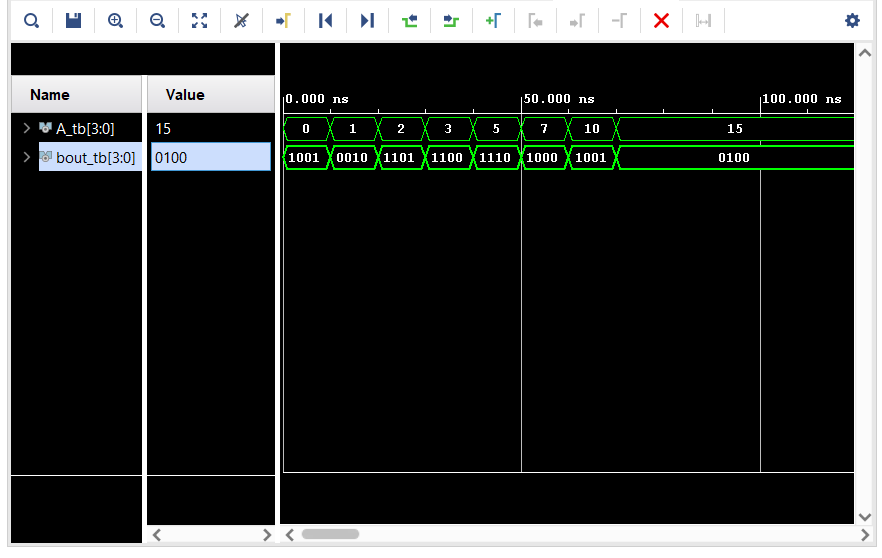
\includegraphics[width=1\textwidth]{img/Sim_Rom_plus_M}
	\caption{Waveform della simulazione di S}
	\label{SchemS} 
\end{figure}
Si procede con dei test effettuati manualmente per mostrare la correttezza nel funzionamento del sistema S. Per consentire una maggiore leggibilità, si è scelto di visualizzare gli indirizzi come \textit{Unsigned Decimal}.\\
Nel caso $A = 0$, si accede alla stringa $00001001$, sommando i bit meno significativi con quelli più significativi si ottiene $0000+1001$ = $1001$;
nel caso $A = 5$, si accede alla stringa $01001010$, e procedendo come sopra si ottiene $0100+1010$ = $1110$.\\
Come si può vedere, i risultati di questi test coincidono con il comportamento atteso dal sistema e che sono mostrati nella waveform relativa alla simulazione. 





